\documentclass{llncs}
% Grundgröße 12pt, zweiseitig
% Standardpakete
% richtiges encoding fuer verschiedene compiler
\usepackage{iftex}
\ifPDFTeX
   \usepackage[utf8]{inputenc}
   \usepackage[T1]{fontenc}
   \usepackage{lmodern}
\else
   \ifXeTeX
     \usepackage{fontspec}
   \else
     \usepackage{luatextra}
   \fi
   \defaultfontfeatures{Ligatures=TeX}
\fi
% deutsche Silbentrennung
\usepackage[english]{babel}
\usepackage{amsmath}
\usepackage{cite}
\usepackage{float}
\usepackage{subfig}
\usepackage{changepage}

% Grafiken einbinden
\usepackage{graphicx}
\graphicspath{{../figures/}}

\usepackage{hyperref}
% tiefe des Inhaltsverzeichnisses
\setcounter{tocdepth}{2}

\usepackage{listings}
\usepackage{color}

\definecolor{dkgreen}{rgb}{0,0.6,0}
\definecolor{gray}{rgb}{0.5,0.5,0.5}
\definecolor{mauve}{rgb}{0.58,0,0.82}

\lstset{frame=tb,
  language=Python,
  aboveskip=3mm,
  belowskip=3mm,
  showstringspaces=false,
  columns=flexible,
  basicstyle={\small\ttfamily},
  numbers=none,
  numberstyle=\tiny\color{gray},
  keywordstyle=\color{blue},
  commentstyle=\color{dkgreen},
  stringstyle=\color{mauve},
  breaklines=true,
  breakatwhitespace=true,
  tabsize=3
}

\begin{document}

\title{Exploration of Abalone game-playing agents}
\author{Ture Claußen, 202132027, \email{ture.claussen@stud.hs-hannover.de}}
\authorrunning{T. Claußen}
\institute{Dept. of Software and Computer Engineering, Ajou University}

% jetzt gehts los
{\def\addcontentsline#1#2#3{}\maketitle} % Wird gebraucht, damit der Title nicht im Inhaltsverzeichnis steht

\begin{abstract}
	Perfect information games provide a good environment for artificial agents to navigate in, as they have a clear performance measure for comparison with each other and humans. Their determinism removes some of the engineering problems of agents in the physical world. In the following we implement and compare alpha-beta pruning and Monte Carlo Tree Search for the game Abalone, to come to a conclusion about their resource-consumption and performance.
	\keywords{AI \and Alpha-beta \and Monte-Carlo-Tree-Search \and Abalone \and Intelligent Agents}
\end{abstract}

\section{Introduction}

Abalone is a fairly new game, that was devised in 1987 by Michel Lalet and Laurent Lévi. Nevertheless, with more than four million global sales it has established itself as a classic game \cite{noauthor_abalone_2020}. Abalone is a two-player game consisting of a hexagonal board with 61 fields and 14 marbles for black and white respectively. The abstract nature of the game requires the player to plan ahead and find the right strategy in the plethora of moves. The goal is to create an agent that is up to par with human players and moreover, has realistic computational requirements and reacts quickly.

In search of the optimal move it is not possible to expand all of the possible paths the game could take, even for modern computers. Hence, more sophisticated approaches for navigating the state space and evaluating good paths are needed. On the other hand, the game does not have piece-specific rules or large distance moves which reduces the need for a very domain specific knowledge about the game like e.g. for chess to find sensible heuristics.

\subsection{Motivation}
Overall, this degree of complexity makes the game a good project for the design of a game playing-agent, as it is meant to be an opportunity to apply the fundamental principles and algorithms learned in the class, as opposed to being distracted by the engineering aspects. This matches my personal background on the subject matter, as I have no prior (formal) exposure to the design of artificial intelligence. In addition, this project is only created for the purpose of this class.

Over the course of my current study of applied computer science I gained versatile proficiency in programming and the handling of data which will help implement the algorithms efficiently and provide the empirical foundation for the paper. The project will also be a valuable training for my upcoming bachelor thesis.

\subsection{Related work}

Considering the existing landscape of papers, there is unquestionably a wide array of papers exploring the application of minimax and alpha-beta pruning on the game of Abalone. Some of the most prominent include:

\begin{enumerate}
	\item "Algorithmic fun-abalone" (2002) Considers foundational heuristics for the game and analyzes minimax and its refinements in the form of (heuristic) alpha-beta pruning. Furthermore it sheds light on the performance differences between those. \cite{aichholzer_algorithmic_2002}
	\item "A Simple Intelligent Agent for Playing Abalone Game: ABLA" (2004) Implementation of a game-playing agent with minimax, alpha-beta pruning and some custom heuristics. The evaluation of the performance is done by comparing the agent to existing software in the form of ABA-PRO and RandomSoft.\cite{ozcan_simple_2004}
	\item "Constructing an abalone game-playing agent" (2005) Provides a very thorough explanation and analysis of the game's fundamentals, such as the state space, rules and positions. In regards to the alpha-beta pruning it also explains strategies for ordering the nodes and performance concerns. \cite{lemmens_constructing_2005}
	\item "Implementing a computer player for abalone using alpha-beta and monte-carlo search" (2009) This master thesis is a very exhaustive analysis of the game, alpha-beta pruning and Monte Carlo tree search, conferring many of the previous results. \cite{chorus_implementing_2009}
\end{enumerate}

These resources give great insight into the classical approaches, but they are lacking certain qualities:
\begin{itemize}
	\item Accessible and freely explorable code that underlies the analysis
	\item Comparison with modern approaches like Q-Learning that might reduce the resource demand on the client side
\end{itemize}

The proposed project seeks to build upon the given insight to improve upon these missing qualities.

\subsection{Rules}
The goal of the game is to push six of the opponent's marbles off the playing field. The game's starting position is depicted in figure \ref{basics} (a). One, two, or three adjacent marbles (of the player's own color) may be moved in any of the six possible directions during a player's turn. We differentiate between broadside or "side-step" moves and "in-line" moves, depending on how the chain of marbles moves relative to its direction, which is shown in figure \ref{basics} (b) and (c).

\begin{figure}[!h]
	\centering
	\subfloat[Starting position]{
		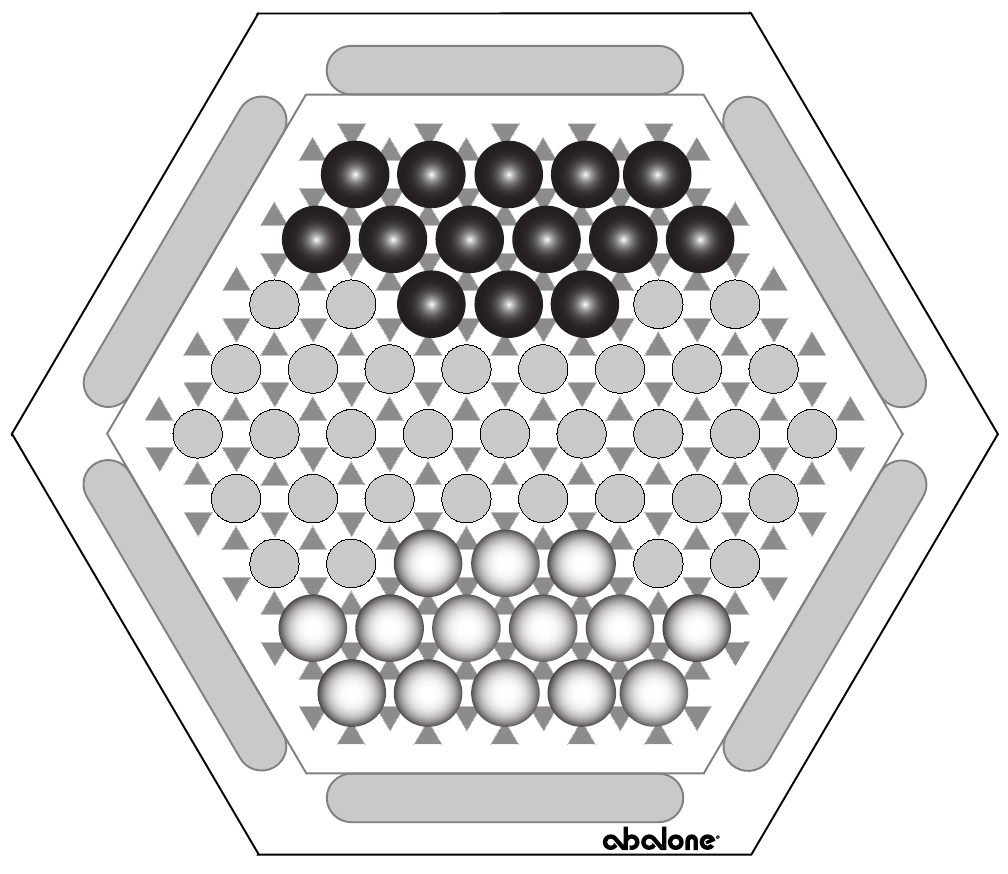
\includegraphics[width=3cm, keepaspectratio]{rules_starting_position.png}
	}
	\hfill
	\subfloat["In-line" moves]{
		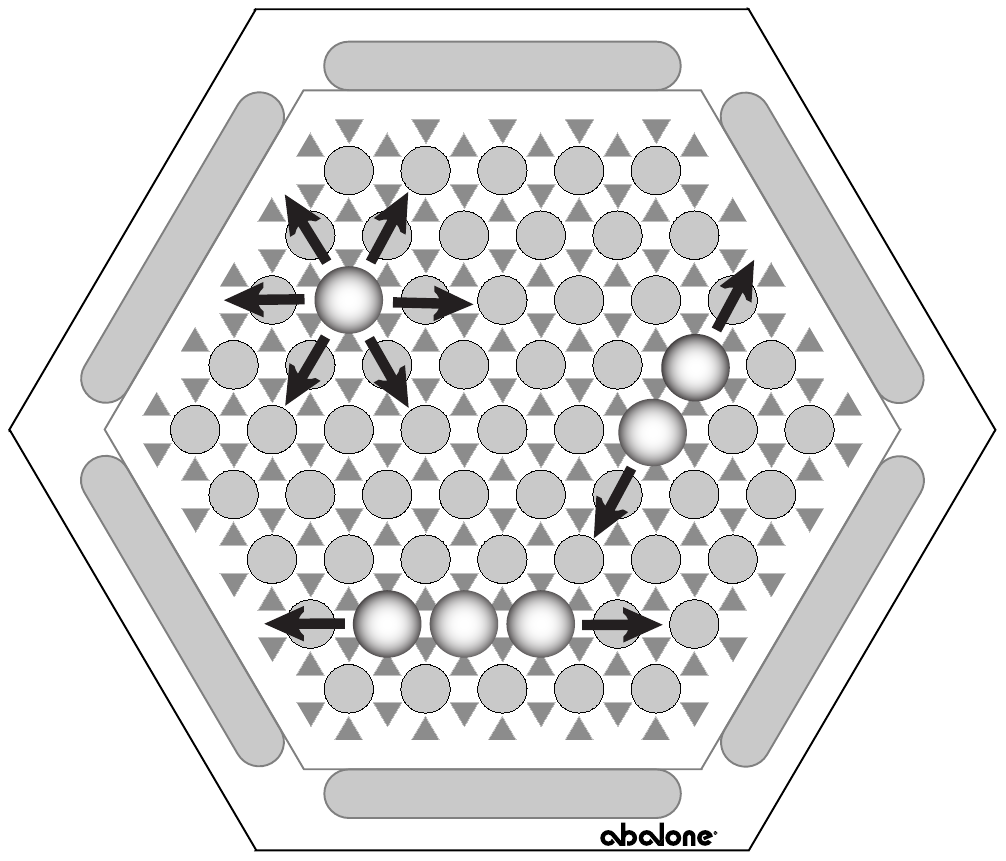
\includegraphics[width=3cm, keepaspectratio]{rules_inline_move.png}
	}
	\hfill
	\subfloat["Side-step" moves]{
		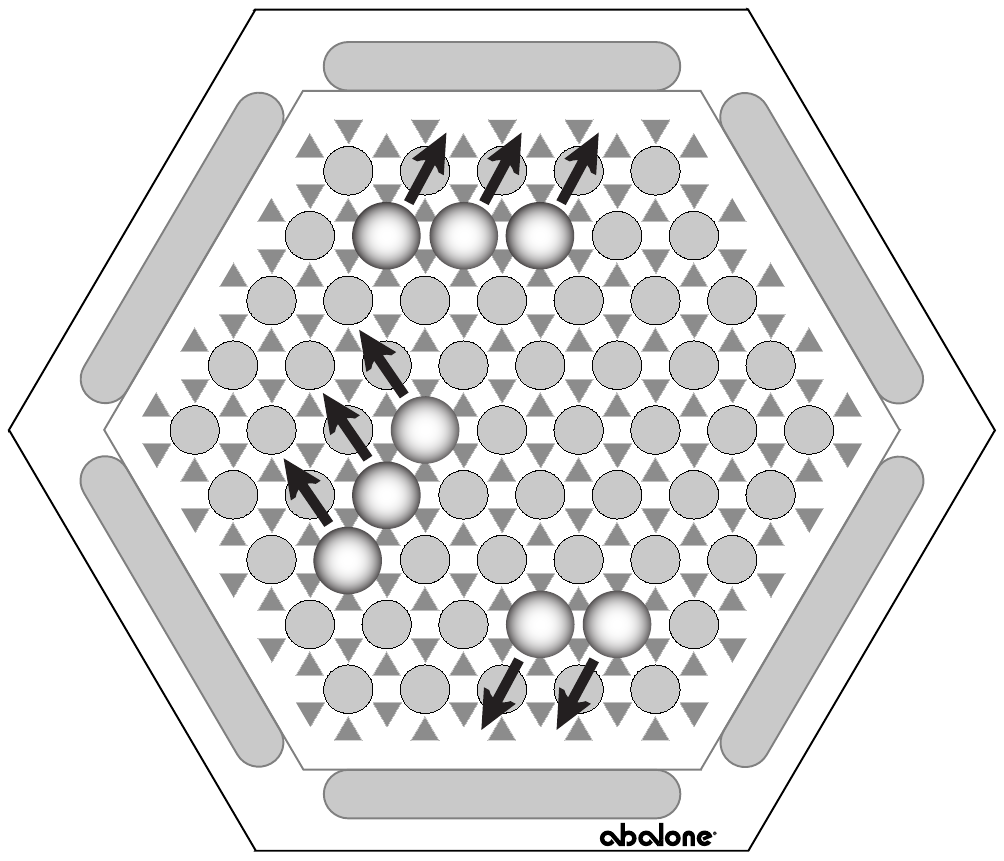
\includegraphics[width=3cm, keepaspectratio]{rules_side_step_move.png}
	}
	\caption{Basic moves \cite{abalone_sa_abalone_nodate}}
	\label{basics}
\end{figure}

A move pushing the opponent's marbles is called "sumito" and comes in three variations, as shown by figure \ref{sumito}. Essentially, the player has to push with superior numbers and the opponent's marbles can not be blocked. This is the game mechanic that allows for pushing the marbles out of the game and winning.

\begin{figure}[!h]
	\centering
	\subfloat["2-push-1" sumito]{
		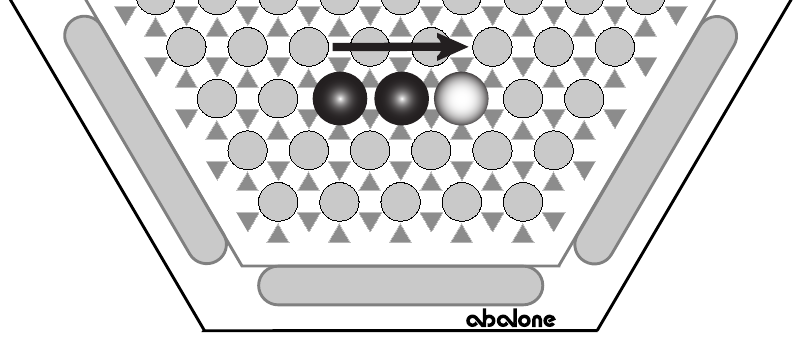
\includegraphics[width=3cm, keepaspectratio]{rules_2-push-1_sumito.png}
	}
	\hfill
	\subfloat["3-push-1" sumito]{
		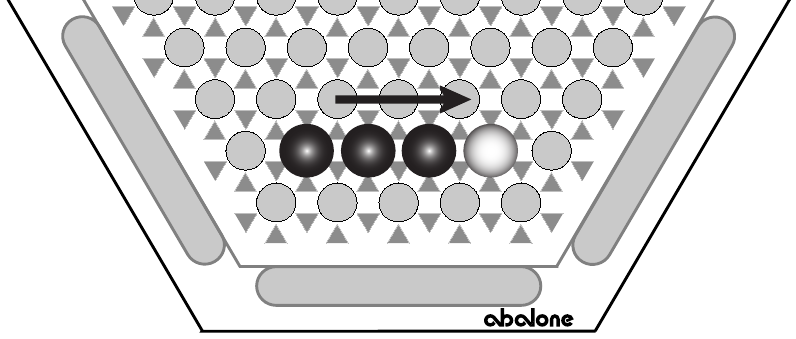
\includegraphics[width=3cm, keepaspectratio]{rules_3-push-1_sumito.png}
	}
	\hfill
	\subfloat["3-push-2" sumito]{
		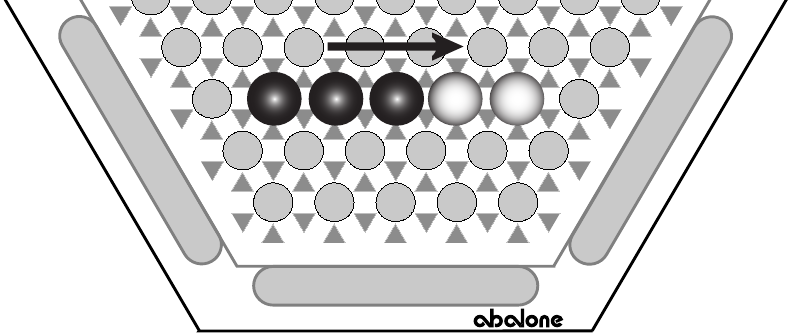
\includegraphics[width=3cm, keepaspectratio]{rules_3-push-2_sumito.png}
	}
	\caption{Sumito positions allow pushing the opponent's marbles \cite{abalone_sa_abalone_nodate}}
	\label{sumito}
\end{figure}

\section{Project details}

\subsection{Agent design}

Based on the PEAS framework we can analyze the task environment for the agent. \cite[p.107]{russell_artificial_2021}

\begin{description}
	\item[Performance measure] Win/loss, number of moves, time to deliberate
	\item[Environment] Digital playing board
	\item[Actuators] Move marbles, display text to CLI
	\item[Sensors] Position of marbles
\end{description}

If we look at the environment more closely we see that it is fully observable, two-agent, competitive, sequential, static and discrete.

\subsection{Complexity}
An important characteristic of a game environment is its complexity, which can be described in two relevant dimensions.

\paragraph{State space complexity}

The state space is the collection of all possible states the agent can be in.\cite[p. 150]{russell_artificial_2021} For Abalone this means we have to consider all possible board configurations with different numbers of marbles present. Additionally, we would have to correct duplicates that arise from the symmetries of the board. Ignoring this fact the following gives a good upper bound:

$$
	\sum_{k=8}^{14}\sum_{m=9}^{14}\frac{61!}{k!(61-k)!}\times\frac{(61-k)!}{m!((61-k)-m)!}
$$

\paragraph{Game tree complexity} The game tree defines the dependencies between board positions (nodes) and moves (edges). First we consider the branching factor (how many moves are possible in one position) of the game tree, which is on average 60. We combine that number with the height of the tree to get the total number of leaves. As the length of a game varies greatly, we use the average length of a game which is 87: $60^{87}$ \cite{lemmens_constructing_2005}

\begin{figure}
	\centering
	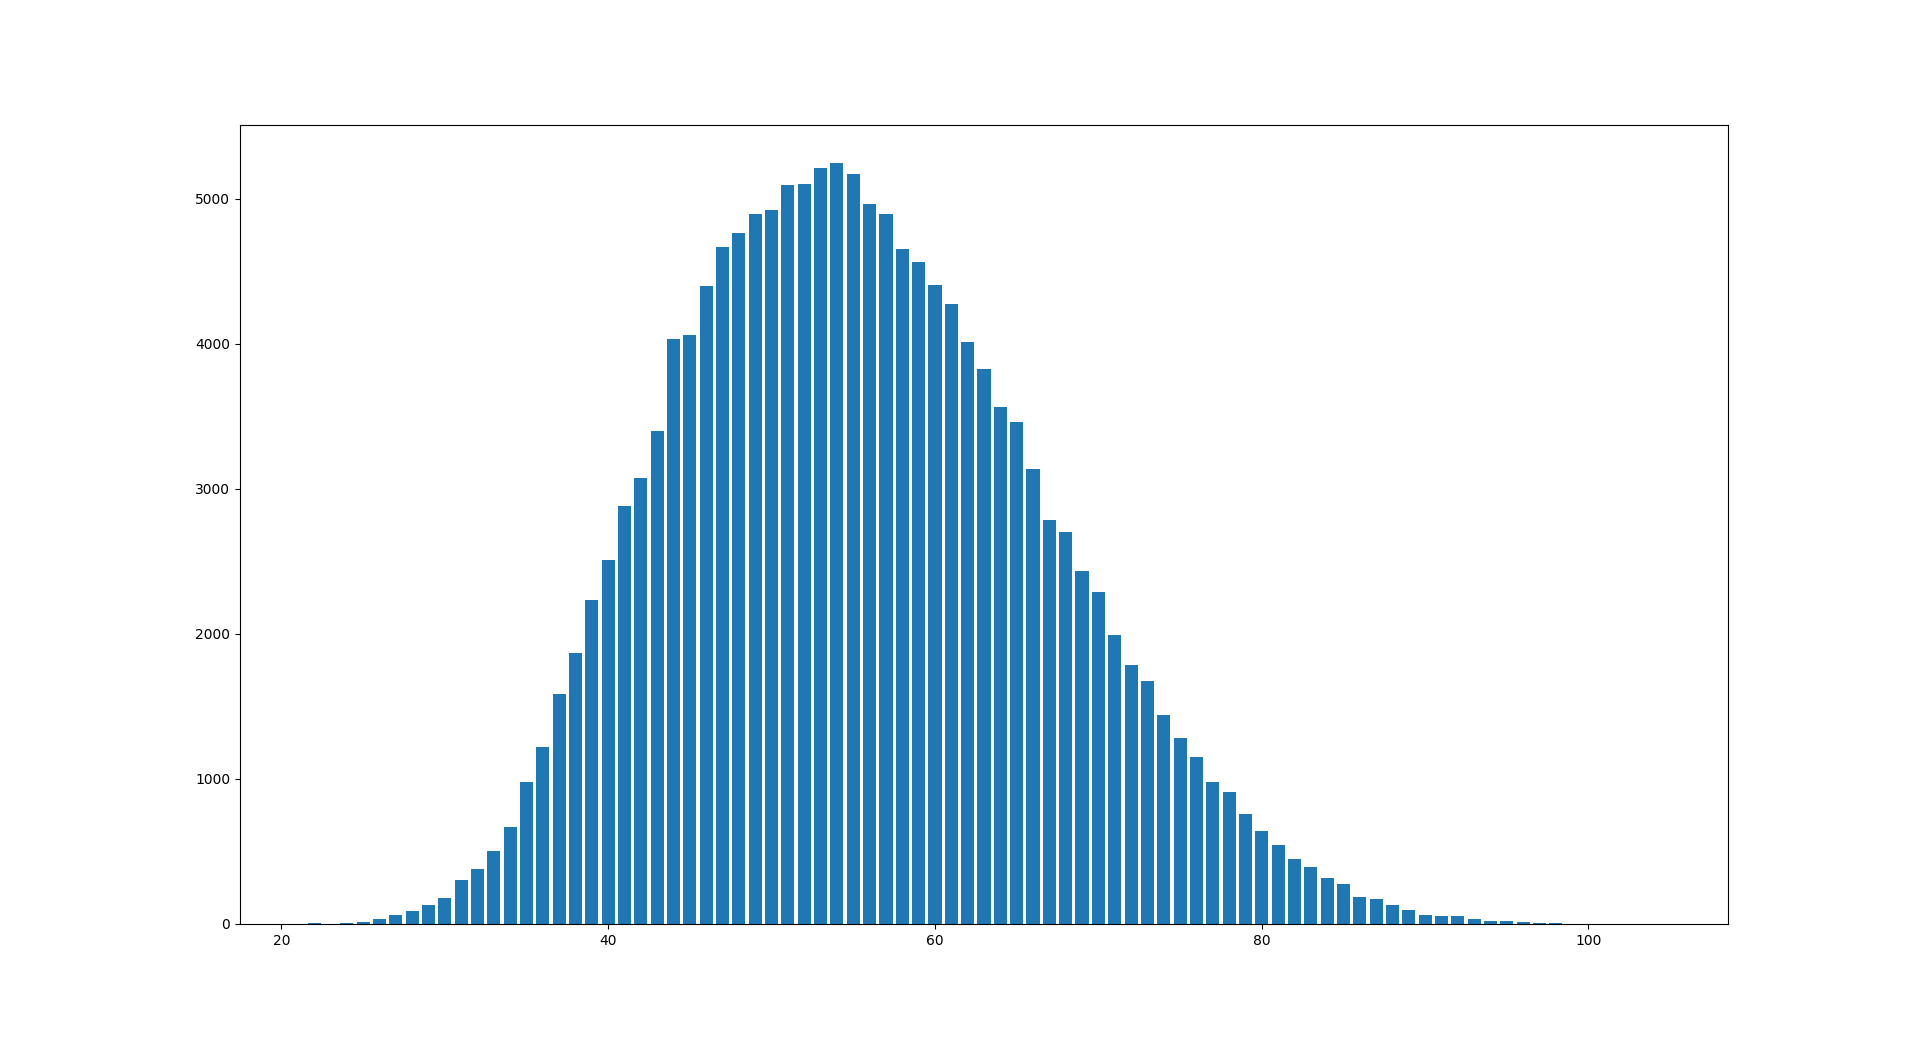
\includegraphics[width=7cm, keepaspectratio]{distribution_of_moves.png}
	\caption{Counts of moves available for random for random player in 5 games}
\end{figure}

Putting Abalone's complexity in relation with other popular games, its state space complexity is on the same level as Reversi, whilst its game tree surpasses chess in complexity (c.f. table \ref{complexity_table})

\begin{table}
	\begin{center}
		\begin{tabular}{ | c | c | c | }
			\hline
			Game        & state-space complexity (log) & game-tree complexity (log) \\
			\hline
			Tic-tac-toe & 3                            & 5                          \\
			\hline
			Reversi     & 28                           & 58                         \\
			\hline
			Chess       & 46                           & 123                        \\
			\hline
			Abalone     & 24                           & 154                        \\
			\hline
			Go          & 172                          & 360                        \\
			\hline
		\end{tabular}
	\end{center}
	\caption{Abalone in comparison with other games \cite{chorus_implementing_2009}}
	\label{complexity_table}
\end{table}


\section{Algorithm design}


\subsection{Heuristics}
As the size of the game tree is very large, the search on the tree usually does not reach terminal leaves that indicate a clear loss or win. Rather one has to evaluate the intermediary result of a given transposition based on a heuristic function. As algorithms like minimax optimize the potential outcome of the next moves based on this function, the heuristics solely determine the performance of such an agent.

This function should judge the positions based on expert knowledge of the game to distinguish good from bad moves.

\paragraph{Adjacency}
As a majority of marbles is required to push opponent's marbles and conversely an equal amount of marbles is needed to avoid being pushed, it can be assumed that keeping one's marbles grouped together is a good move. The measure of adjacency is calculated by iterating over all marbles and counting the directly neighboring marbles that have the same color. We sum up these counts for each player and measure the difference:
$$ \text{adjacency} = n_{\text{self}} - n_{\text{opponent}} $$

This puts the two counts into a relation and produces a negative sign, when the opponent has the upper hand.

% image on how to calculate

\paragraph{Distance to center}
Marbles that are close to the brink of the board put them into danger of being attacked, wherefore it is generally good to place all of the marbles into the center of the board. For each player's marbles we measure their distance from the center of the board as the smallest amount of moves it would take to reach the center (Manhattan distance). Then again we sum up the distances and weigh them against each other to get the final measure:


For both measures it is more convenient to represent the internal array indices of the marbles in a different coordinate system that has better mathematical properties. In case of the hexagonal shape of the board a cube grid or an axial are very suitable.

\begin{figure}[!h]
	\centering
	\subfloat[Axial grid coordinate system]{
		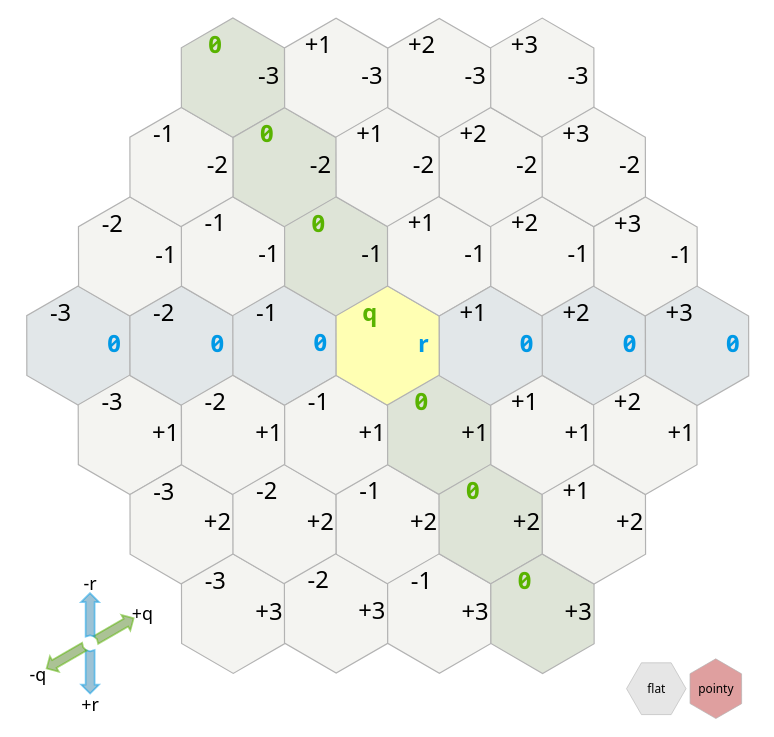
\includegraphics[width=5cm, keepaspectratio]{hex_axial_grid.png}
	}
	\hfill
	\subfloat[Cube grid coordinate system]{
		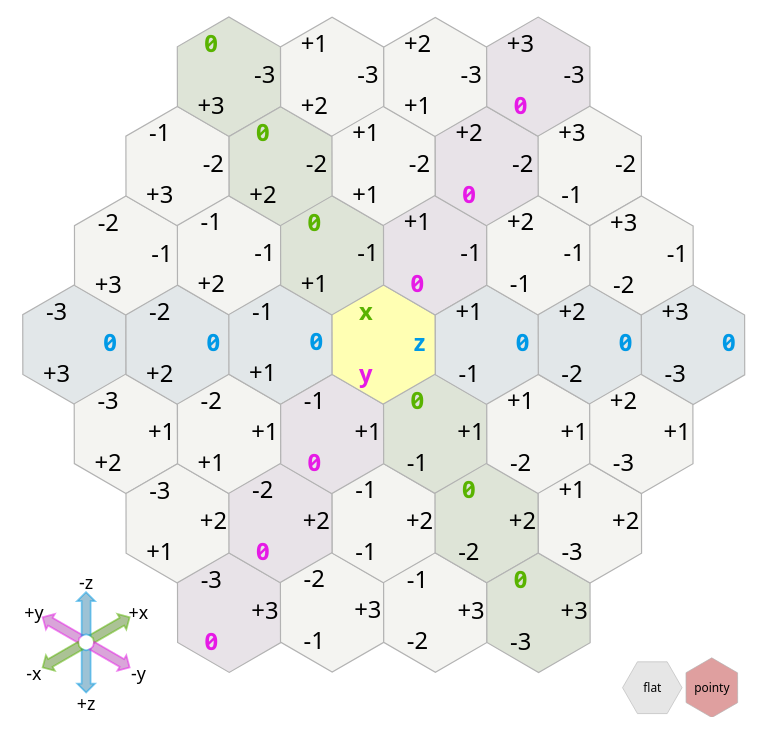
\includegraphics[width=5cm, keepaspectratio]{hex_cube_grid.png}
	}
	\caption{Different options for hexagonal grids \cite{noauthor_red_nodate}}
	\label{hex_grids}
\end{figure}

That way we can obtain the neighbors by just incrementing and decrementing our x-, y- and z-components.

\begin{figure}
	\begin{lstlisting}
  DIRECTIONS = {
    (+1, 0, -1): Direction.NORTH_EAST,
    (+1, -1, 0): Direction.EAST,
    (0, -1, +1): Direction.SOUTH_EAST,
    (-1, 0, +1): Direction.SOUTH_WEST,
    (-1, +1, 0): Direction.WEST,
    (0, 1, -1): Direction.NORTH_WEST
  }
\end{lstlisting}
	\label{directions}
	\caption{Movements mapped to required increments and decrements}
\end{figure}

The same goes for calculating the distance which becomes in this space much more intuitive \ref{distance}.

\begin{figure}
	\begin{lstlisting}
    def distance(self, other: Cube) -> int:
        return max(abs(self.x - other.x), abs(self.y - other.y), abs(self.z - other.z))
\end{lstlisting}
	\label{distance}
	\caption{Code to calculate the distance between two cube coordinates \cite{noauthor_ture_nodate}}
\end{figure}

\paragraph{Score}
By comparing the current configuration of the board to following states in the search tree we can obtain a count of how many marbles were lost and how many were won and again weigh those against each other.

$$ \text{marbleRatio} = n_{\text{won}} - n_{\text{lost}} $$

\paragraph{Win and loss}
Lastly as a more definitive measure we can indicate whether the current state is a terminal state and hence a winning or losing state.

$$ \text{winLoss} =
	\begin{cases}
		1 \text{ if game won } \\
		-1 \text{ otherwise}
	\end{cases}
$$

\subsection{Alpha-beta-pruning agent}
Alpha-beta-pruning is an improvement of the minimax algorithm, that tries to eliminate unnecessary traversals down the search tree, which, in the best case, leads to a reduction of moves from $ O(b^d) $ to $ O(\sqrt{b^d}) $. The implementation of the alpha beta agent could be improved in several ways.

The heuristic function is a linear combination of the above mentioned heuristics was implemented as a linear combination:

\begin{table}
	\begin{center}
		\begin{tabular}{ | c | c | }
			\hline
			Heuristic   & weight \\
			\hline
			adjacency   & 1      \\
			\hline
			distance    & -1.5   \\
			\hline
			marbleRatio & 100    \\
			\hline
			winLoss     & 100000 \\
			\hline
		\end{tabular}
	\end{center}
	\caption{Weights for the linear combination}
	\label{heuristic_table}
\end{table}
\paragraph{Move ordering}
To increase the likelihood of pruning taking place we need to order the moves, such that for the maximizer the best moves come first and for the minimizer vice versa. What constitutes a good move is determined by the heuristic function. That means our move ordering has to be predictive of the resulting heuristic evaluation of the move.

Two different approaches were tested. The first one was based one the following hierarchy:

\begin{itemize}
	\item Move capturing marble: +3
	\item Move pushing marble: +1
	\item Move involving 2/3 marbles: +1/+2
\end{itemize}

Evaluating this function is computationally much less expensive than calculating the full heuristic function so this approach was tried first (Evaluation 1). In comparison to the algorithm without any ordering the visited nodes could be reduced drastically. Depending on the composition of the heuristic the node count for this ordering fluctuates significantly. If we compared it to the approach of using the heuristic itself for ordering, we see that this decreases the node count even further (c.f. table \ref{node_count}). A possible explanation for that would be, the more predictive the move ordering is of the final heuristic the less nodes are visited.

\begin{table}
	\begin{center}
		\begin{tabular}{ | c | c | c | c | c | }
			\hline
			Depth & Without ordering & Evaluation 1 & Evaluation 2 & $\sqrt{b^d}$ \\
			\hline
			1     & 45               & 45           & 45           & 8            \\
			\hline
			2     & 1594             & 304          & 132          & 60           \\
			\hline
			3     & 9755             & 4971         & 2423         & 464          \\
			\hline
			4     & 457309           & 94650        & 6918         & 3600         \\
			\hline
		\end{tabular}
	\end{center}
	\caption{Nodes visited with/without move ordering and the optimal case}
	\label{node_count}
\end{table}

\paragraph{Transposition table}
Due to the nature of abalone there are multiple ways to reach the same configuration of the board. If we save the final value for a state determined by the algorithm, we can potentially save node visits if we visit that node again. To encode the board configurations efficiently, Zobrist Hashing \cite{noauthor_zobrist_nodate} was used. We hold a table with 9 x 9 entries (only 61 of 81 used) and within the cell we hold another 2 cells for the distinct game pieces (black and white marbles). In each cell we store a 64 bit random string.

For each marble on the board we use the indices of the positions on the board to retrieve a bitstring from our table and connect them with XOR to retrieve our final hash $h$.

\paragraph{Branch cutting}
A problem with abalone is that for each configuration there are many possible moves (high branching factor) and many of those possible moves are very bad. If we have a sensible move ordering we might potentially exclude many of the useless moves to have a faster agent. For this implementation we only include at most the first 30 first moves from the ordered list.

\begin{table}
	\begin{center}
		\begin{tabular}{ | c | c | c | c | c | }
			\hline
			Depth & Without TT & With TT & With TT and cutting & $\sqrt{b^d}$ \\
			\hline
			1     & 45         & 45      & 31                  & 8            \\
			\hline
			2     & 132        & 132     & 90                  & 60           \\
			\hline
			3     & 2432       & 2423    & 1019                & 464          \\
			\hline
			4     & 6918       & 5829    & 2435                & 3600         \\
			\hline
		\end{tabular}
	\end{center}
	\caption{Nodes visited with/without transposition table, branch cutting and the optimal case}
	\label{node_count}
\end{table}

\paragraph{Further improvement}
At this point the choice of the library also becomes relevant. Even though the reduction of node visits brings the most noticable difference in time for deliberation, the implementation can make a significant impact as well. There are two components of the game library that are called extremely often and thereby heavily profit from performance improvements.

For one that is the routine to generate all possible moves. For each node expansion this function is called. By forking the game library \cite{campfireman_campfiremanabalone-boai_2021} and making improvements to that function the execution time could be reduced to 10\% of its original value. Furthermore, a tradeoff between execution time and memory was made, by storing and updating the current positions of the marbles, instead of iterating the entire board array.

\subsection{Monte Carlo Search agent}
Monte Carlo Tree Search promises to improve on some of the pitfalls posed by alpha-beta/minimax by allowing for a greater search depth and not using a heuristic function. In its simplest/purest form moves are evaluated by performing a playout, simulating the game until its end. The playout policy for selecting the moves in the playout is in its simplest form random move selection.

Due to the large set of possible moves, the selection of random moves as playout policy has bad performance especially when the number of simulations is limited to a relatively small $n$. For the pure implementation we get about 1000 simulations when the move time is limited to 20 seconds.

\paragraph{UCB}
Whereas in the pure implementation each move gets an equal amount of simulations, we can select the next node to expand based on how promising the node(n) it is. We normalize the utility $U(n)$ by the number of games $N(n)$. By considering how often a node and its parent have been visited already, we want them to be visited more often in the beginning, before we solely decide based on utility. For this implementation a $ C = \sqrt{2}$ was chosen. \cite[p.327 ff]{russell_artificial_2021}

$$
	UCB(n) = \frac{U(n)}{N(n)} + C \times \sqrt{\frac{\log{N(Parent(n))}}{N(n)}}
$$

\paragraph{Playout policy}
Ideally, we want the players in the simulations to make very good decisions for their moves such that the playout's result is very meaningful. In order to achieve that the Evaluation 1 function from above was used to order the moves and expand only the best moves. This comes at a great computational cost, almost halving the amount of simulations but potentially improving the quality.

\paragraph{Other improvements}
Again by making adjustments to the game library significant performance improvements could be made. Namely by creating a new function for the generation of a random move. Instead of creating all possible moves and then selecting a random one, a random move is generated directly.

\subsection{Algorithm comparison}
As follows the results of different pairings of algorithms and their variations.

\begin{table}
	\begin{adjustwidth}{-5in}{-5in}% adjust the L and R margins by 1 inch
		\begin{center}
			\begin{tabular}{ | c | c | c | c | c | c | c | c | }
				\hline
				Black player               & White player        & \small{Marbles lost b} & \small{Marbles lost w} & \small{time p. move b} & \small{time p. move w} & \small{total moves (avg)} & n \\
				\hline
				AlphaBeta (d=3)            & Random              & 0.2                    & 6.0                    & 11.11                  & 0.0                    & 57.6                      & 5 \\
				\hline
				AlphaBeta (d=4)            & Random              & 0.0                    & 6.0                    & 142.8                  & 0.0                    & 52.4                      & 5 \\
				\hline
				AlphaBeta (d=3)            & AlphaBetaFast (d=3) & 6.0                    & 5.0                    & 10.02                  & 4.16                   & 92                        & 1 \\
				\hline
				MonteCarloPure (t=20s)     & RandomPlayer        & 5.0                    & 0.0                    & 20.33                  & 0.0                    & 1008.0                    & 1 \\
				\hline
				MonteCarloImproved (t=20s) & RandomPlayer        & 0.0                    & 6.0                    & 20.05                  & 0.0                    & 306.0                     & 1 \\
				\hline
				MonteCarloImproved (t=20s) & AlphaBetaFast (d=3) & 0.0                    & 6.0                    & 69.0                   & 20.06                  & 6.24                      & 1 \\
				\hline
			\end{tabular}
		\end{center}
		\label{node_count}
	\end{adjustwidth}
	\medskip% adds some space after the table
	\caption{Face-off results}
\end{table}

\section{Conclusion}
Overall, the implementation of the agents posed a much greater engineering challenge than expected. The basic algorithms were implemented quickly, but two tweak them until they have acceptable move-times required a lot of effort. It is interesting that the basic implementation of the Monte Carlo Search agents performed so poorly. Especially, combined with more modern techniques the MCTS agent still is extremely promising and worth further investigation.


% Literatur
\bibliographystyle{splncs04.bst}
\bibliography{../ref.bib}
\end{document}